\documentclass[14pt,a4paper]{extbook}
\usepackage[T5]{fontenc}
\usepackage[utf8]{inputenc}
\usepackage[vietnamese]{babel}
\usepackage{amsmath, amssymb}
\usepackage{enumitem}
\usepackage{geometry}
\usepackage{graphicx}
\usepackage{caption}
\usepackage[most]{tcolorbox}
\usepackage{setspace}

\geometry{margin=1in}
\onehalfspacing  % hoặc \doublespacing cho dòng đôi

\newenvironment{problem}[1][]{
  \par\noindent\textbf{Bài #1.}\ \ignorespaces
}{\par}

\begin{document}

\chapter{Tính chất của số học}
\section{Vì sao bắt đầu bằng số học?}

Con đã biết cộng, trừ, nhân, chia. Thậm chí con còn có thể giải
được nhiều bài trong chương này rồi. Vậy tại sao chúng ta lại mở
đầu cuốn sách bằng \emph{cả một chương} nói về số học?

Để trả lời, ta quay lại tên sách: \emph{Tiền đại số}. \emph{Tiền
đại số} là gì? Có nhiều cách hiểu khác nhau, nhưng chúng mình
(những người viết sách) xem \emph{tiền đại số} là chiếc cầu nối
giữa \emph{số học} và \emph{đại số}.

\emph{Số học} là những điều căn bản: cộng, trừ, nhân, chia, và có
thể thêm vài điều thú vị như bình phương hay căn bậc hai. Có lẽ
con đã học phần lớn những điều này rồi. Điều thường làm con thấy
khó nhất trong số học là \emph{bài toán bằng lời}, ví dụ: “Lan có
$5$ quả táo, Minh có $7$ quả, hỏi cả hai bạn có tất cả bao nhiêu
quả?” Khi lớn hơn, các số có thể to hơn, nhưng kiểu bài thì không
khó hơn bao nhiêu. Số học rất giỏi khi giải những việc đơn giản
như đếm đồ vật. 

Nhưng khi bài toán trở nên \emph{phức tạp} hơn — như tính đường
bay của tên lửa, phân tích thị trường tiền tệ, hay đếm xem có bao
nhiêu cách để một tin nhắn đi qua các trạm thu phát — ta cần một
“hộp dụng cụ” mạnh mẽ hơn.

“Hộp dụng cụ” đó là \emph{đại số}. Đại số là ngôn ngữ của toán
học nâng cao. Đại số cho ta những công cụ để lấy ý tưởng từ số học
và biến chúng thành các quy tắc \emph{khái quát}, nghĩa là ta có
thể dùng các ý tưởng ấy không chỉ cho bài toán số học, mà còn cho
rất nhiều dạng bài khác nữa.

Ta hãy xem một ví dụ đơn giản. Dùng số học, ta có thể chứng minh rằng:
\[
2\times(3+5)=(2\times3)+(2\times5).
\]
Vì vế trái là $2\times8=16$, còn vế phải là $6+10=16$. Hai bên bằng nhau.

Nhưng đại số cho ta một quy tắc tổng quát hơn:
\[
a\times(b+c)=(a\times b)+(a\times c),
\]
đúng với mọi số $a,b,c$. Trong toán học cao hơn, $a,b,c$ có thể không
chỉ là các số quen thuộc, mà có thể là những đối tượng toán học phức
tạp hơn. (Và khi đó, dấu “$+$” hay “$\times$” có thể mang ý nghĩa khác
với phép cộng và phép nhân thông thường — nhưng điều đó ta sẽ học sau.)

Mục tiêu ban đầu trong chương này là đặt ra những quy tắc cơ bản của
số học, và giúp con hiểu \emph{vì sao} chúng lại đúng. Khi nắm được
các quy tắc ấy, con sẽ sẵn sàng bắt đầu tư duy theo hướng đại số.

\subsection*{Vì sao cần hiểu “vì sao”?}
Khi đọc đến đây, con đã đủ lớn để không chỉ biết \emph{làm thế nào}
để tính, mà còn muốn biết \emph{vì sao} cách tính đó lại đúng. Hiểu
vì sao toán học hoạt động như thế là chìa khóa để giải được các bài
toán khó hơn. Nếu con chỉ biết cách bấm máy hoặc làm theo công thức mà
không hiểu bản chất, thì khi gặp bài khác lạ, con sẽ rất khó sửa đổi
hay mở rộng cách làm đó. Vì vậy, trong cuốn sách này, thầy cô sẽ không
chỉ nói “làm thế này để ra kết quả”, mà sẽ luôn cố gắng chỉ ra “vì sao
nó đúng”.

\subsection*{Kết thúc chương này, con sẽ biết giải thích vì sao:}
\begin{itemize}
  \item $(-5)\times(-7)=35$ (và không phải $-35$).
  \item $(1990\times1991)-(1989\times1990)=3980$ (và có thể nhẩm được!).
  \item $8\div\tfrac{1}{7}=56$.
  \item $(4\times10\times49)\div(2\times5\times7)=28$ (cũng nhẩm được!).
\end{itemize}

Con sẽ hiểu tất cả những điều này không phải vì học thuộc lòng công
thức, mà vì hiểu được toán học ẩn bên trong các phép tính đó.

\subsection*{Một chút lưu ý}
Đôi khi, các nhà toán học ở những nơi khác nhau dùng từ hơi khác nhau
cho cùng một ý. Giống như người Mỹ gọi là “truck” còn người Anh gọi là
“lorry”, nhưng cùng chỉ chiếc xe tải. Vì thế, trước khi học tiếp, ta
sẽ thống nhất một số từ để dùng trong cuốn sách này cho rõ ràng nhé.


Hình dưới là \emph{đường số}. Đường số kéo dài mãi về hai phía.
Mỗi vạch nhỏ chỉ một \emph{số nguyên}. Ta thấy các số
\[
\ldots,-6,-5,-4,-3,-2,-1,0,1,2,3,4,5,6,\ldots
\]

\begin{figure}[ht!]
  \centering
  % Dùng bản PDF khi biên dịch LaTeX
  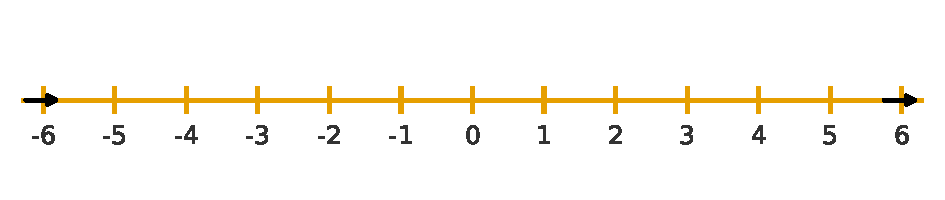
\includegraphics[width=0.9\textwidth]{img/fig-numberline.pdf}
  \caption*{\small Đường số với các vạch từ $-6$ đến $6$ và mũi tên chỉ rằng
  đường số còn kéo dài nữa.}
\end{figure}

\noindent\textbf{Tên gọi đơn giản:}
\begin{itemize}
  \item \textit{Số dương}: đứng bên phải $0$.
  \item \textit{Số âm}: đứng bên trái $0$.
  \item \textit{Không âm}: là số dương hoặc $0$.
  \item \textit{Không dương}: là số âm hoặc $0$.
  \item \textit{Khác $0$}: mọi số trừ $0$.
\end{itemize}

\begin{quote}
\textbf{Ghi chú:} Có nơi gọi \emph{số tự nhiên} là $1,2,3,\ldots$,
có nơi tính cả $0$. Trong tài liệu này, ta dùng: \emph{số nguyên dương}
cho $1,2,3,\ldots$ và \emph{số nguyên không âm} cho $0,1,2,\ldots$.
\end{quote}


\section{Phép cộng}

Ta bắt đầu với phép toán quen thuộc nhất: \emph{phép cộng}.
Tuy đơn giản, nhưng hiểu rõ tính chất của phép cộng sẽ giúp con
tính nhẩm nhanh và làm chủ các phép tính phức tạp hơn.

\begin{problem}[1.1]
Dựa vào \emph{hai hình vẽ} bên dưới, hãy giải thích vì sao
$2+3=3+2$.

\begin{figure}[ht!]
  \centering
  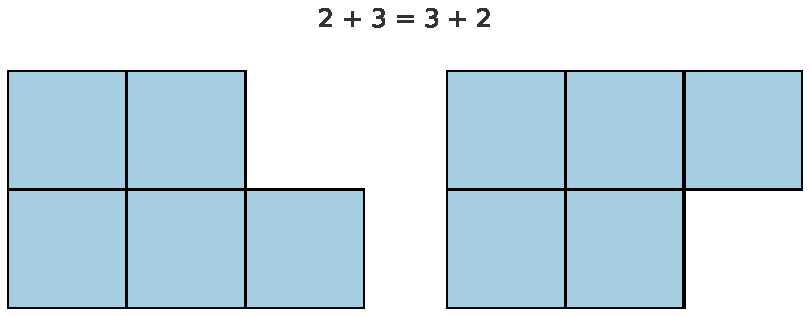
\includegraphics[width=0.55\textwidth]{img/fig-prob1.1.pdf}
  \caption*{\small Gợi ý: đổi chỗ hai nhóm ô vuông, tổng vẫn không đổi.}
\end{figure}
\end{problem}

\begin{problem}[1.2]
Dựa vào \emph{hai hình vẽ} bên dưới, hãy giải thích vì sao
$(2+3)+4=2+(3+4)$.

\begin{figure}[ht!]
  \centering
  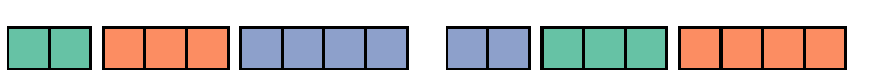
\includegraphics[width=0.55\textwidth]{img/fig-prob1.2.pdf}
  \caption*{\small Gợi ý: cộng nhóm đầu tiên hay nhóm sau đều cho cùng tổng.}
\end{figure}
\end{problem}

\begin{problem}[1.3]
\begin{enumerate}[label=(\alph*)]
  \item Dùng các tính chất ở trên, giải thích:
  \[
  472+(219+28)=(472+28)+219.
  \]
  \item Tính nhẩm $472+(219+28)$.
  \begin{flushright}\small(Nguồn: MATHCOUNTS)\end{flushright}
\end{enumerate}
\end{problem}

\begin{problem}[1.4]
Tính:
\[
(2+12+22+32)+(8+18+28+38).
\]
\begin{flushright}\small(Nguồn: MATHCOUNTS)\end{flushright}
\end{problem}

\begin{problem}[1.5]
Tính tổng:
\[
1+2+3+\cdots+19+20.
\]
\textit{Gợi ý:} Dấu \texttt{$\cdots$} nghĩa là ta cộng tất cả số theo
mẫu từ $1$ đến $20$.
\end{problem}


\begin{problem}[1.6]
Dựa vào hình dưới đây, hãy giải thích vì sao $2 + 0 = 2$.

\begin{figure}[ht!]
  \centering
  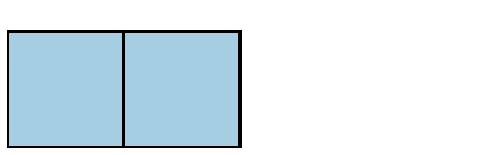
\includegraphics[width=0.55\textwidth]{img/fig-prob1.6.pdf}
  \caption*{\small Hai ô vuông cộng với “không ô vuông” vẫn bằng hai ô vuông.}
\end{figure}
\end{problem}

\begin{problem}[1.1]
Dựa vào hai hình bên dưới, hãy giải thích vì sao $2 + 3 = 3 + 2$.

\begin{figure}[ht!]
  \centering
  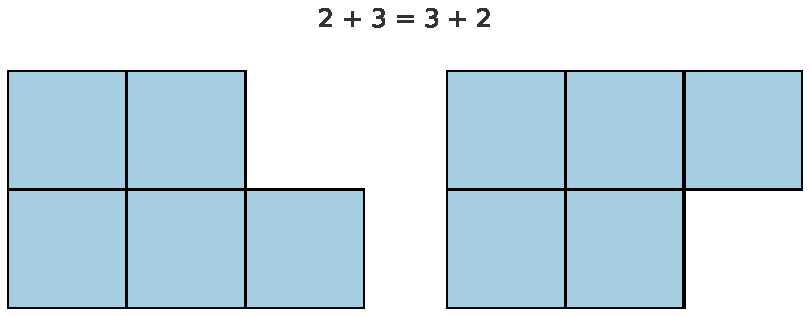
\includegraphics[width=0.55\textwidth]{img/fig-prob1.1.pdf}
  \caption*{\small Hai cách sắp xếp khác nhau của cùng số ô vuông.}
\end{figure}

\textbf{Lời giải:}  
Trước hết, hãy nhìn vào hình bên trái. Hàng đầu tiên có $2$ ô vuông, hàng thứ hai có $3$ ô vuông.  
Tổng cộng là $2 + 3$ ô vuông.  

Bây giờ, nhìn sang hình bên phải. Hàng đầu tiên có $3$ ô vuông, hàng thứ hai có $2$ ô vuông.  
Tổng cộng cũng là $3 + 2$ ô vuông.  

Hình bên phải thực ra chỉ là bản lật ngược của hình bên trái.  
Lật ngược hình không làm thay đổi số lượng ô vuông.  
Do đó, ta kết luận rằng:
\[
2 + 3 = 3 + 2.
\]
\end{problem}

Mỗi khi chúng ta cộng hai số, \textbf{thứ tự} của các số không làm thay đổi kết quả.  
Ví dụ:
\[
5 + 17 = 17 + 5, \quad 32 + 999 = 999 + 32.
\]
Có vô số ví dụ như vậy.  
Tất nhiên, ta không thể viết hết ra được, nên ta dùng cách viết tổng quát hơn:
\[
\text{số thứ nhất} + \text{số thứ hai} = \text{số thứ hai} + \text{số thứ nhất.}
\]

Để ngắn gọn, ta gọi số thứ nhất là $a$, số thứ hai là $b$.  
Khi đó, ta có:
\[
a + b = b + a.
\]

Ở đây, $a$ và $b$ có thể là bất kỳ số nào (hoặc có thể bằng nhau).  
Ví dụ, nếu $a = 2$ và $b = 3$, ta có $2 + 3 = 3 + 2$.  
Nếu $a = 100$ và $b = 200$, ta có $100 + 200 = 200 + 100$.  

Chữ $a$ và $b$ được gọi là \emph{biến} (hay \emph{ẩn}), vì giá trị của chúng có thể thay đổi tuỳ từng bài toán.

\begin{quote}
\textbf{Tính chất giao hoán của phép cộng:}  
Với mọi số $a$ và $b$, ta luôn có
\[
a + b = b + a.
\]
\end{quote}

Trong Bài 1.1, ta đã thấy $a + b = b + a$ là đúng khi $a = 2$, $b = 3$.  
Nhưng một ví dụ riêng lẻ chưa đủ để chứng minh rằng công thức này đúng với \emph{mọi} số $a$ và $b$.  
Để làm được điều đó, ta sẽ học thêm nhiều bước lập luận chặt chẽ hơn ở các chương sau.

Bây giờ ta đã hiểu rằng thứ tự của hai số khi cộng không làm thay đổi kết quả.
Vậy nếu ta cộng \emph{ba} số thì sao?

\begin{problem}[1.2]
Dựa vào hai hình dưới đây, hãy giải thích vì sao
\[
(2 + 3) + 4 = 2 + (3 + 4).
\]

\begin{figure}[ht!]
  \centering
  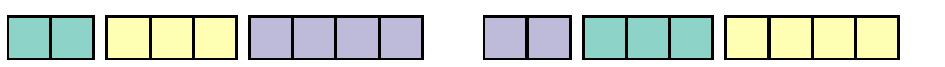
\includegraphics[width=0.75\textwidth]{img/fig-prob1.2-assoc.pdf}
  \caption*{\small Hai cách nhóm khác nhau của ba nhóm ô vuông.}
\end{figure}
\end{problem}

\noindent\textbf{Gợi ý:} Dấu ngoặc cho biết ta cần tính phần nào trước.
Ví dụ, $(3 + 4) \times 5$ nghĩa là $7 \times 5$, trong khi $(4 \times 5)$ nghĩa là $3 + 20$.


\textbf{Lời giải cho Bài 1.2:}  
Với mỗi hình, ta sẽ đếm số ô vuông sáng, rồi đếm số ô vuông tối, sau đó cộng hai kết quả lại.

- Trong hình bên trái: có $(2 + 3)$ ô sáng và $4$ ô tối.  
  Tổng cộng có $(2 + 3) + 4$ ô vuông.

- Trong hình bên phải: có $2$ ô sáng và $(3 + 4)$ ô tối.  
  Tổng cộng có $2 + (3 + 4)$ ô vuông.

Điểm khác nhau duy nhất giữa hai hình là màu của hàng ở giữa.  
Việc đổi màu không làm thay đổi số ô, nên ta kết luận:
\[
(2 + 3) + 4 = 2 + (3 + 4).
\]

Từ đây, ta có thể viết quy tắc tương tự cho bất kỳ ba số nào:
\[
(a + b) + c = a + (b + c).
\]
Nói cách khác, nếu ta cộng $a$ và $b$ trước rồi cộng $c$,  
hay cộng $b$ và $c$ trước rồi cộng $a$, thì kết quả vẫn như nhau.  
Tính chất này gọi là \textbf{tính chất kết hợp của phép cộng.}

\begin{quote}
\textbf{Tính chất kết hợp của phép cộng:}  
Với mọi số $a, b, c$, ta luôn có:
\[
(a + b) + c = a + (b + c).
\]
\end{quote}

\begin{tcolorbox}[colback=yellow!10!white,colframe=orange!80!black,title={Lưu ý quan trọng}]
Học sinh đôi khi nhầm giữa hai tính chất “\emph{giao hoán}” và “\emph{kết hợp}”.  
Trong \textbf{tính chất giao hoán}, ta \emph{đổi chỗ} các số (ví dụ $a+b=b+a$).  
Trong \textbf{tính chất kết hợp}, ta \emph{nhóm} các số khác nhau  
(ví dụ $(a+b)+c=a+(b+c)$), nhưng không đổi vị trí của chúng.
\end{tcolorbox}

%----------------------------------------
% 1.3  Quy tắc đổi chỗ + kết hợp giúp cộng theo "bất kỳ thứ tự"
%----------------------------------------

\paragraph{Gộp lại,} hai tính chất \emph{giao hoán} và \emph{kết hợp}
mạnh mẽ hơn ta tưởng. Chúng cho phép ta cộng một dãy số theo \emph{bất
kỳ thứ tự} nào. Bài tiếp theo minh hoạ nguyên tắc “cộng theo mọi thứ
tự” này.

\begin{problem}[1.3]
\begin{enumerate}[label=(\alph*)]
  \item Dùng các tính chất ở Bài 1.1 và 1.2, hãy giải thích vì sao
  \[
    472 + (219 + 28) \;=\; (472 + 28) + 219.
  \]
  \item Tính tổng \(\;472 + (219 + 28)\).
  \begin{flushright}\small(Nguồn: MATHCOUNTS)\end{flushright}
\end{enumerate}
\end{problem}

\noindent\textbf{Lời giải cho Bài 1.3:}

\smallskip
\noindent(a)\; Ta bắt đầu từ vế trái:
\[
  472 + (219 + 28).
\]
Ta muốn biến đổi để nó trông giống vế phải. Trước hết, ta \emph{đổi
chỗ} \(219\) và \(28\) ở trong ngoặc nhờ tính chất giao hoán, tức là
thay \((219+28)\) bởi lượng bằng nó là \((28+219)\):
\[
  472 + (219 + 28) \;=\; 472 + (28 + 219).
\]
Biểu thức này đã gần giống điều ta cần: \((472 + 28) + 219\).
Thực ra hai biểu thức đó \emph{bằng nhau} nhờ tính chất kết hợp, vì ta
được phép \emph{đổi cách nhóm} các số hạng:
\[
\begin{aligned}
  472 + (219 + 28) 
  &= 472 + (28 + 219) && \text{(giao hoán)}\\
  &= (472 + 28) + 219 && \text{(kết hợp).}
\end{aligned}
\]

\smallskip
\noindent(b)\; Từ phần (a), hai biểu thức
\(472 + (219 + 28)\) và \((472 + 28) + 219\) là bằng nhau, nên ta có
thể tính \((472 + 28) + 219\) thay vì tính trực tiếp.
Nhẩm \(472 + 28 = 500\). Vậy ta còn lại \(500 + 219\),
nên kết quả là \(719\).

\medskip
\noindent\(\square\)

\medskip
\noindent\textbf{Điều quan trọng của Bài 1.3:} Ta có thể \emph{sắp xếp
lại} các số trong phép cộng để phép tính trở nên \emph{dễ} hơn. Thường
thì thuận tiện nhất là ghép những số “đẹp” với nhau trước (ví dụ làm
tròn trăm), rồi mới cộng phần còn lại. Trong thực hành, ta sẽ không
viết lại toàn bộ các bước như ở Bài 1.3 mỗi lần. Thay vào đó, ta vận
dụng hiểu biết về \emph{tính chất giao hoán} và \emph{tính chất kết
hợp} để tự do sắp xếp, nhóm lại các số theo cách tốt nhất. Hãy áp dụng
nguyên tắc này cho bài tiếp theo nhé!

%----------------------------------------
% 1.4  Ghép cặp để tính nhanh hơn
%----------------------------------------
\begin{problem}[1.4]
Tính:
\[
(2 + 12 + 22 + 32) + (8 + 18 + 28 + 38).
\]
\begin{flushright}\small(Nguồn: MATHCOUNTS)\end{flushright}
\end{problem}

\noindent\textbf{Lời giải cho Bài 1.4:}  
Ta có thể bắt đầu cộng từng số, nhưng như vậy sẽ mất nhiều thời gian.  
Thay vào đó, hãy sắp xếp lại các số sao cho mỗi cặp có cùng tổng.  
Cụ thể, ta ghép mỗi số ở nhóm thứ nhất với một số ở nhóm thứ hai như sau:
\[
(2 + 38) + (12 + 28) + (22 + 18) + (32 + 8).
\]
Mỗi cặp đều có tổng bằng \(40\).  
Vì có bốn cặp, nên tổng bằng:
\[
40 + 40 + 40 + 40 = 160.
\]
Vậy kết quả là \(\boxed{160}.\)
\medskip

---

%----------------------------------------
% 1.5  Cộng dãy số dài bằng cách ghép cặp
%----------------------------------------
\begin{problem}[1.5]
Tính tổng:
\[
1 + 2 + 3 + \cdots + 19 + 20.
\]
\textit{Gợi ý:} Dấu \texttt{$\cdots$} nghĩa là ta cộng tất cả các số theo mẫu,  
nên ở đây ta cộng các số nguyên dương từ 1 đến 20.
\end{problem}

\noindent\textbf{Lời giải cho Bài 1.5:}  
Chúng ta chắc chắn không muốn cộng lần lượt 20 số đâu!  
Hãy thử ghép các số thành cặp để mỗi cặp có cùng tổng.  
Ta ghép số nhỏ nhất với số lớn nhất, số nhỏ thứ hai với số lớn thứ hai, v.v.:
\[
(1 + 20) + (2 + 19) + (3 + 18) + \cdots + (10 + 11).
\]
Ta có 20 số, tức là 10 cặp.  
Mỗi cặp đều bằng \(21\).  
Vậy tổng là:
\[
21 + 21 + 21 + 21 + 21 + 21 + 21 + 21 + 21 + 21.
\]
Cộng 10 lần 21 tức là \(10 \times 21 = 210.\)
\[
\boxed{210}.
\]

---

%----------------------------------------
% 1.6  Cộng thêm số 0
%----------------------------------------
\begin{problem}[1.6]
Dựa vào hình dưới đây, hãy giải thích vì sao \(2 + 0 = 2.\)

\begin{figure}[ht!]
  \centering
  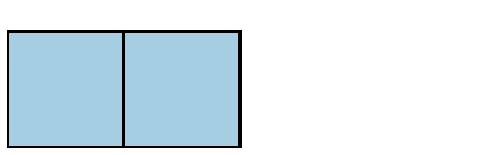
\includegraphics[width=0.4\textwidth]{img/fig-prob1.6.pdf}
  \caption*{\small Hai ô vuông cộng với “không ô vuông” vẫn là hai ô vuông.}
\end{figure}
\end{problem}

\noindent\textbf{Lời giải cho Bài 1.6:}  
Một mặt, ta có 2 ô vuông.  
Mặt khác, có thể nói rằng ta có 2 ô sáng và 0 ô tối.  
Vì vậy ta được phương trình:
\[
2 + 0 = 2.
\]
Khi cộng thêm số 0 vào bất kỳ số nào, kết quả vẫn không thay đổi.

\begin{tcolorbox}[colback=yellow!10!white, colframe=orange!80!black,
title={Tính chất cộng với số không}]
Nếu \(a\) là một số bất kỳ, thì:
\[
a + 0 = a.
\]
\end{tcolorbox}

%============================
% BÀI TẬP CUỐI MỤC 1.2
%============================
\subsection*{Bài tập}
\begin{enumerate}[label=1.2.\arabic*.]
  \item Tính \(99+99+99+101+101+101\).
  \item Tính \(1999+2001+1999+2001+1999+2001+1999+2001\).
  \item Tính \((3+13+23+33+43)+(7+17+27+37+47)\).
  \item Tính \((1+2+3+\cdots+49+50)+(99+98+97+\cdots+51+50)\).
\end{enumerate}

%============================
% 1.3  PHÉP NHÂN
%============================
\section{Phép nhân}

\noindent Ta bắt đầu khám phá phép toán tiếp theo: \emph{phép nhân}.
Ta sẽ dùng hình ảnh để thấy vì sao các quy tắc của phép nhân là đúng.

%----------------------------
\begin{problem}[1.7]
Dựa vào \emph{hai hình} dưới đây, hãy giải thích vì sao \(2\times3=3\times2\).

\begin{figure}[ht!]
  \centering
  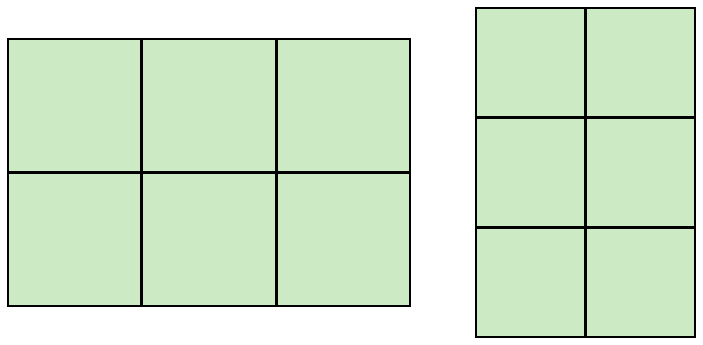
\includegraphics[width=0.50\textwidth]{img/fig-prob1.7.pdf}
  \caption*{\small Hai lưới ô vuông: \(2\) hàng \(\times\) \(3\) cột và \(3\) hàng \(\times\) \(2\) cột.
  Số ô đều bằng \(6\).}
\end{figure}

\textbf{Gợi ý:} Đếm số ô theo “số hàng nhân số cột”. Đổi chỗ hàng–cột
không làm thay đổi số ô. Đây chính là \emph{tính chất giao hoán của phép nhân}.
\end{problem}

%----------------------------
\begin{problem}[1.8]
Bằng cách đếm các chấm trong \emph{một hình} theo \emph{hai cách}, hãy giải thích vì sao
\[
(2\times3)\times4 \;=\; 2\times(3\times4).
\]

\begin{figure}[ht!]
  \centering
  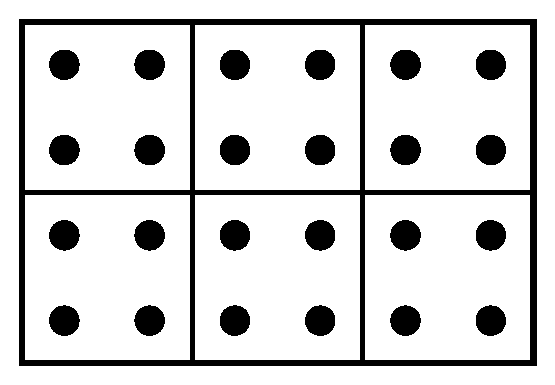
\includegraphics[width=0.25\textwidth]{img/fig-prob1.8.pdf}
  \caption*{\small Một dãy chấm gồm \(2\) hàng và \(12\) cột. Các vạch đứt
  phân chia thành \(4\) nhóm, mỗi nhóm \(3\) cột.}
\end{figure}

\textbf{Gợi ý:} 
\begin{itemize}
  \item Nhóm theo cột trước: có \(4\) nhóm, mỗi nhóm \(2\times3\) chấm
  \(\Rightarrow (2\times3)\times4\).
  \item Hoặc gộp tất cả: \(2\) hàng và \(3\times4=12\) cột
  \(\Rightarrow 2\times(3\times4)\).
\end{itemize}
Hai cách đếm cho cùng kết quả \(\Rightarrow\) \emph{tính chất kết hợp của phép nhân}.
\end{problem}

%----------------------------
\begin{problem}[1.9]
Tính \(25\times125\times4\times6\times8\).
\end{problem}

%----------------------------
\begin{problem}[1.10]
Dựa vào \emph{hình} dưới đây, hãy giải thích vì sao \(2\times1=2\).

\begin{figure}[ht!]
  \centering
  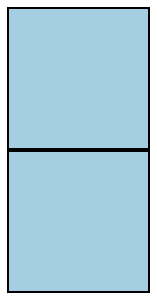
\includegraphics[width=0.10\textwidth]{img/fig-prob1.10.pdf}
  \caption*{\small Một cột gồm \(2\) ô vuông: \(2\) hàng, \(1\) cột.}
\end{figure}

\textbf{Gợi ý:} \(2\times1\) nghĩa là “\(2\) hàng, mỗi hàng có \(1\) ô”,
nên tổng cộng có \(2\) ô.
\end{problem}

%----------------------------
\begin{problem}[1.11]
\begin{enumerate}[label=(\alph*)]
  \item Tính \((5+6)\times7\).
  \item Tính \(5+(6\times7)\).
\end{enumerate}
\end{problem}

%============================
% Các bài tiếp theo của mục 1.3
%============================

\begin{problem}[1.12]
Dựa vào \emph{hình} dưới đây, hãy giải thích vì sao
\[
2\times(3+4) \;=\; (2\times3) + (2\times4).
\]

\begin{figure}[ht!]
  \centering
  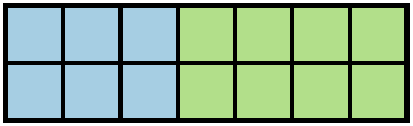
\includegraphics[width=0.75\textwidth]{img/fig-prob1.12.pdf}
  \caption*{\small Hình chữ nhật \(2\) hàng \(\times\) \(7\) cột.
  Ba cột đầu tô một màu (ứng với \(2\times3\)),
  bốn cột sau tô màu khác (ứng với \(2\times4\)).}
\end{figure}
\end{problem}

\begin{problem}[1.13]
Tính \(51\cdot9 + 51\cdot31\).
\end{problem}

\begin{problem}[1.14]
Giá trị của \(17\cdot13 + 51\cdot13 + 32\cdot13\) bằng bao nhiêu?
\end{problem}

\begin{problem}[1.15]
Xét các phép nhân sau:
\[
\begin{aligned}
5\times 7 &= 35\\
4\times 7 &= 28\\
3\times 7 &= 21\\
2\times 7 &= 14\\
1\times 7 &= 7\\
0\times 7 &=\ \underline{\hspace{2cm}}
\end{aligned}
\]
\begin{enumerate}[label=(\alph*)]
  \item Tìm \emph{quy luật} trong các kết quả phép nhân.
  \item Giả sử quy luật đó tiếp tục đúng, hãy dự đoán kết quả phép nhân cuối.
\end{enumerate}
\end{problem}

%============================
% Nhắc lại Bài 1.7 và lời giải
%============================
\begin{problem}[1.7]
Dựa vào \emph{hai hình} bên dưới, hãy giải thích vì sao \(2\times3=3\times2\).

\begin{figure}[ht!]
  \centering
  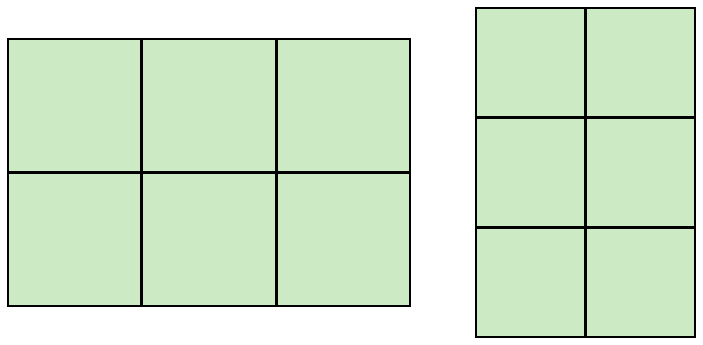
\includegraphics[width=0.50\textwidth]{img/fig-prob1.7.pdf}
  \caption*{\small Hai lưới: \(2\) hàng \(\times\) \(3\) cột và \(3\) hàng \(\times\) \(2\) cột.
  Đếm số ô cho kết quả như nhau.}
\end{figure}
\end{problem}

\noindent\textbf{Lời giải cho Bài 1.7:}  
Hình bên trái có \(2\) hàng, mỗi hàng \(3\) ô, nên tổng số ô là \(3+3\),
tức \(2\times3\).  
Hình bên phải có \(3\) hàng, mỗi hàng \(2\) ô, nên tổng số ô là \(2+2+2\),
tức \(3\times2\).  
Hình bên phải chỉ là \emph{phiên bản xoay} của hình bên trái. Xoay hình
không làm thay đổi số ô. Vì vậy ta kết luận \(2\times3=3\times2\).

Ví dụ này gợi ý rằng ta có thể \emph{đổi chỗ} hai số trong phép nhân
giống như trong phép cộng. Nói cách khác, phép nhân có \emph{tính chất
giao hoán}. Giống như phép cộng, đây chưa phải là một chứng minh tổng
quát cho mọi số, nhưng ví dụ cho ta trực giác tốt về vì sao quy tắc này
đúng với các số dương \(a,b\). Ta viết ngắn gọn:
\[
a\times b \;=\; b\times a.
\]
Ta gọi đó là \textbf{tính chất giao hoán của phép nhân}.

%------------------------------------------------------------
% Nhân: kí hiệu, giao hoán, kết hợp — và Bài 1.8
%------------------------------------------------------------

\paragraph{Kí hiệu phép nhân.}
Ta thường viết \(a\times b\) thành \(a\cdot b\) (dấu chấm ở giữa).
Lí do: viết dấu chấm nhanh hơn, và dấu “\(\times\)” dễ bị nhầm với
chữ \(x\) trong đại số. Vì vậy, với mọi số \(a,b\) ta có thể viết
\(a\cdot b=b\cdot a\).

Đôi khi, ta còn viết gọn hơn nữa: bỏ dấu chấm và ghi liền \(ab\).
Cách này còn nhanh hơn. Tuy nhiên không phải lúc nào cũng được bỏ
dấu chấm. Chẳng hạn \(3\cdot4\) không thể viết thành \(34\), vì
\(34\) là một số khác. Khi cần, ta có thể viết \(3\cdot4\) hoặc
\(3(4)\) để chỉ phép nhân.

\begin{tcolorbox}[colback=yellow!10, colframe=orange!80!black,
title={Quan trọng: Phép nhân có tính \emph{giao hoán}}]
Cho \(a\) và \(b\) là các số. Khi đó
\[
ab = ba.
\]
\end{tcolorbox}

\paragraph{Phép nhân có tính kết hợp không?}
Ví dụ sau hơi “mẹo” hơn một chút.

\begin{problem}[1.8]
Bằng cách đếm số chấm trong hình dưới đây theo \emph{hai cách khác nhau},
hãy giải thích vì sao
\[
(2\times3)\times4 = 2\times(3\times4).
\]

\begin{figure}[h!]
  \centering
  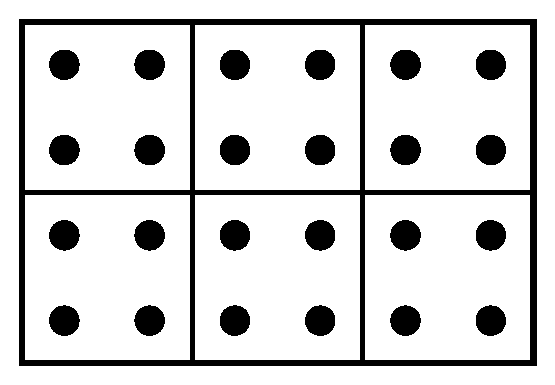
\includegraphics[width=0.25\textwidth]{img/fig-prob1.8.pdf}
  \caption*{\small Một bảng \(2\times3\) “ô”, mỗi ô có 4 chấm.}
\end{figure}
\end{problem}

\noindent\textbf{Lời giải cho Bài 1.8.}
Một mặt, hình có \((2\times3)\) ô; mỗi ô có \(4\) chấm. Vậy tổng số chấm là
\((2\times3)\times4\).

Mặt khác, có \(2\) hàng ô. Mỗi hàng có \((3\times4)\) chấm. Vậy tổng số chấm là
\(2\times(3\times4)\).

Ta đã đếm \emph{cùng một} hình theo hai cách và được cùng kết quả. Suy ra
\[
(2\times3)\times4 = 2\times(3\times4).
\]
\(\square\)

\begin{tcolorbox}[colback=yellow!10, colframe=orange!80!black,
title={Quan trọng: Phép nhân có tính \emph{kết hợp}}]
Cho \(a,b,c\) là các số. Khi đó
\[
(ab)c = a(bc).
\]
\end{tcolorbox}

\paragraph{Kết luận.}
Cùng nhau, tính chất \emph{giao hoán} và \emph{kết hợp} cho phép ta nhân
nhiều số theo \emph{bất kì thứ tự} nào, giống như khi cộng. Kể cả khi có
hơn ba số, nguyên tắc “nhân theo mọi thứ tự/nhóm” vẫn áp dụng. Ở phần sau,
ta sẽ thấy điều này hoạt động ra sao trong tính toán.

%============================
% Bài 1.9
%============================
\begin{problem}[1.9]
Tính \(25 \times 125 \times 4 \times 6 \times 8\).
\end{problem}

\noindent\textbf{Lời giải cho Bài 1.9:}
Nhân \(25\times125\) trực tiếp sẽ khá vất vả, nên ta sắp xếp lại các số
để phép tính gọn hơn. Hãy ghép các cặp “đẹp” như \(4\times25\) và
\(8\times125\). Chẳng hạn:
\[
6 \times (4\times25) \times (8\times125).
\]
Ta có \(4\times25=100\) và \(8\times125=1000\).
Do đó,
\[
6 \times 100 \times 1000 = 600{,}000.
\]
Vậy đáp án là \(\boxed{600{,}000}\). \(\square\)

%============================
% Bài 1.10
%============================
\begin{problem}[1.10]
Dựa vào \emph{hình} dưới đây, hãy giải thích vì sao \(2\times1=2\).
\begin{figure}[ht!]
  \centering
  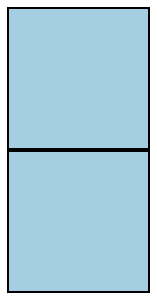
\includegraphics[width=0.10\textwidth]{img/fig-prob1.10.pdf}
  \caption*{\small Một cột gồm \(2\) ô vuông: \(2\) hàng, \(1\) cột.}
\end{figure}
\end{problem}

\noindent\textbf{Lời giải cho Bài 1.10:}
Nhìn theo một cách, có \(2\) hàng; mỗi hàng có \(1\) ô vuông, nên tổng cộng
là \(2\times1\) ô. Nhìn theo cách khác, rõ ràng có đúng \(2\) ô. Vì vậy
\(2\times1=2\). \(\square\)

Ví dụ này cho thấy: \emph{nhân một số với \(1\) không làm thay đổi số đó}.
Từ đây ta có quy tắc sau:

\begin{tcolorbox}[colback=yellow!10, colframe=orange!80!black,
title={Quan trọng: Nhân với số \(1\)}]
Cho \(a\) là một số bất kỳ. Khi đó
\[
1a = a.
\]
\end{tcolorbox}

%============================
% Chuyển tiếp sang kết hợp phép tính
%============================
Trước khi tiếp tục với các tính chất khác, ta cần hiểu cách \emph{kết hợp
nhiều phép tính} trong cùng một biểu thức. Nếu chỉ cộng hoặc chỉ nhân,
ta có thể đổi chỗ và nhóm số theo mọi thứ tự. Nhưng khi vừa có cộng vừa
có nhân, mọi thứ sẽ phức tạp hơn một chút. Ví dụ, \(5+6\times7\) có ý
nghĩa gì?

%============================
% Bài 1.11
%============================
\begin{problem}[1.11]
\begin{enumerate}[label=(\alph*)]
  \item Tính \((5+6)\times7\).
  \item Tính \(5+(6\times7)\).
\end{enumerate}
\end{problem}

\noindent\textbf{Lời giải cho Bài 1.11:}

\noindent(a)\; Dấu ngoặc cho biết ta phải cộng trước:
\[
(5+6)\times7 \;=\; 11\times7 \;=\; 77.
\]

% (Phần (b) sẽ được trình bày ở trang sau của tài liệu gốc.)

%====================================================
% Tiếp theo Bài 1.11(b) và Quy tắc thứ tự thực hiện
%====================================================

\noindent\textbf{(b)} Lần này, dấu ngoặc cho biết ta phải \emph{nhân trước}:
\[
5 + (6\times7) \;=\; 5 + 42 \;=\; 47.
\]

Ta thấy rằng \((5+6)\times7 \;\neq\; 5 + (6\times7)\). (Kí hiệu “\(\neq\)”
nghĩa là “không bằng”.)

Vậy nếu chỉ cho biểu thức \(\;5 + 6\times7\;\) mà \emph{không có} dấu ngoặc
thì làm thế nào? Ta cần một bộ quy tắc để biết \emph{thứ tự} thực hiện các
phép tính. (Đến giờ ta mới học cộng và nhân; các phép khác sẽ bàn ở sau.)

\begin{tcolorbox}[colback=yellow!10, colframe=orange!80!black,
title={Quan trọng: Thứ tự thực hiện phép tính}]
Thực hiện các phép trong một biểu thức theo thứ tự sau:
\begin{enumerate}
  \item Tính các biểu thức \textbf{trong ngoặc} trước.
  \item Tính \textbf{lũy thừa}. (Sẽ học ở Chương~2.)
  \item \textbf{Nhân và chia} từ trái sang phải.
  \item \textbf{Cộng và trừ} từ trái sang phải.
\end{enumerate}
\end{tcolorbox}

Vì vậy, để tính \(\;5 + 6\times7\;\), ta \textbf{nhân trước}, rồi mới cộng:
\[
5 + 6\times7 \;=\; 5 + 42 \;=\; \mathbf{47}.
\]
Nói cách khác, phép tính này giống như phần (b) của Bài 1.11.

%====================================================
% Dẫn vào quy tắc phân phối với ví dụ trực quan
%====================================================

Tiếp theo, ta đến một quy tắc rất mạnh \emph{kết nối} phép cộng và phép nhân.
Như thường lệ, ta sẽ dùng một ví dụ đơn giản để tạo trực giác trước.

\begin{problem}[1.12]
Dựa vào \emph{hình} dưới đây, hãy giải thích vì sao
\[
2\times(3+4) \;=\; (2\times3) + (2\times4).
\]

\begin{figure}[ht!]
  \centering
  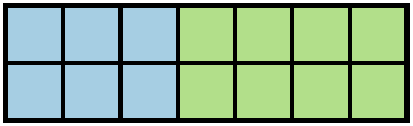
\includegraphics[width=0.80\textwidth]{img/fig-prob1.12.pdf}
  \caption*{\small Hình chữ nhật \(2\) hàng \(\times\) \(7\) cột.
  Ba cột đầu tô một màu (ứng với \(2\times3\)),
  bốn cột sau tô màu khác (ứng với \(2\times4\)).}
\end{figure}
\end{problem}

\noindent\textbf{Lời giải cho Bài 1.12:}
Nhìn theo một cách, có \(2\) hàng, mỗi hàng có \((3+4)\) ô.
Vậy tổng là \(2\times(3+4)\).

Nhìn theo cách khác, có \((2\times3)\) ô màu đậm và \((2\times4)\) ô màu nhạt.
Vậy tổng là \((2\times3) + (2\times4)\).

Ta đã đếm \emph{cùng một} hình theo hai cách khác nhau, nên kết luận:
\[
2\times(3+4) \;=\; (2\times3) + (2\times4).
\]
\(\square\)

%====================================================
% Quy tắc phân phối của phép nhân (tiếp theo) và Bài 1.13
%====================================================

\paragraph{Ví dụ 1.12} cho ta một quy tắc rất hữu ích nối phép nhân với
phép cộng. Với ba số bất kỳ \(a,b,c\), ta có
\[
a\times(b+c)=(a\times b)+(a\times c).
\]
Nói cách khác, \emph{phép nhân được “phát đều”} vào hai phần của phép
cộng. Vì thế, quy tắc này được gọi là \textbf{tính chất phân phối của
phép nhân đối với phép cộng}, hay ngắn gọn là \emph{tính chất phân phối}.

Do phép nhân \emph{giao hoán}, ta cũng có thể viết khi tổng đứng \emph{trước}:
\[
(b+c)\times a=(b\times a)+(c\times a).
\]
Để gọn hơn, ta thường viết phép nhân bằng dấu chấm hoặc viết liền:
\(ab\) nghĩa là \(a\cdot b\).

\begin{tcolorbox}[colback=yellow!10, colframe=orange!80!black,
title={Quan trọng: Phép nhân \emph{phân phối} qua phép cộng}]
Cho \(a,b,c\) là các số. Khi đó
\[
a(b+c)=ab+ac
\qquad\text{và}\qquad
(b+c)a=ba+ca.
\]
Hai công thức trên thực chất là \emph{một} quy tắc, chỉ khác nhau ở việc
tổng đứng trước hay đứng sau.
\end{tcolorbox}

Bây giờ ta luyện tập thêm với quy tắc phân phối. Nó giúp được gì cho ta?

%----------------------------
\begin{problem}[1.13]
Tính \(51\cdot9 + 51\cdot31\).
\end{problem}

\noindent\textbf{Lời giải cho Bài 1.13:}
Thay vì tính riêng \(51\cdot9\) và \(51\cdot31\), ta dùng tính chất phân phối:
\[
51\cdot9 + 51\cdot31 \;=\; 51\,(9+31).
\]
Vế phải có \(9+31=40\), nên kết quả bằng \(51\cdot40\).

Ta lại dùng tính chất phân phối để nhân cho gọn: viết \(51=50+1\),
\[
51\cdot40=(50+1)\cdot40=50\cdot40+1\cdot40.
\]
Hai tích này đều “đẹp”: \(50\cdot40=2000\) và \(1\cdot40=40\).
Vậy
\[
50\cdot40+1\cdot40=2000+40=2040.
\]
Kết quả là \(\boxed{2040}\). \(\square\)

%====================================================
% Phân phối hai chiều - Khai triển và Đưa thừa số chung ra ngoài
%====================================================

Như ta đã thấy ở Bài 1.13, ta có thể dùng tính chất phân phối
\emph{theo cả hai chiều}. Dùng tính chất phân phối để biến
\(a(b+c)\) thành \(ab+ac\) gọi là \emph{khai triển}. Ngược lại, dùng
tính chất phân phối để biến \(ab+ac\) thành \(a(b+c)\) gọi là
\emph{đưa thừa số chung ra ngoài} (rút gọn theo thừa số chung).

Ví dụ, ở bước đầu của lời giải Bài 1.13, ta đã “đưa thừa số chung”
từ \(51\cdot9+51\cdot31\) thành \(51(9+31)\).
Ở bước sau, ta “khai triển” \((50+1)\cdot40\) thành \(50\cdot40+1\cdot40\).

\begin{tcolorbox}[colback=blue!3,colframe=blue!60!black,title={Góc ý tưởng: Đưa thừa số chung}]
\textbf{Đưa thừa số chung} nghĩa là dùng tính chất phân phối để viết
một biểu thức dạng \(ab+ac\) thành \(a(b+c)\).
\[
51\cdot9+51\cdot31 \;=\; 51\,(9+31).
\]
Trong ví dụ này, \(51\) là \emph{thừa số chung}. Ta nói “đưa \(51\) ra
ngoài” hay “rút \(51\) làm thừa số chung”.
\end{tcolorbox}

Đến đây, ta mới dùng tính chất phân phối với tổng của \emph{hai} số hạng.
Vậy với tổng dài hơn thì sao?

%----------------------------
\begin{problem}[1.14]
Giá trị của \(17\cdot13 + 51\cdot13 + 32\cdot13\) bằng bao nhiêu?
\end{problem}

\noindent\textbf{Lời giải cho Bài 1.14 (cách 1, theo từng bước):}
Ta biết có thể dùng tính chất phân phối nếu hai tích có cùng một thừa số
chung (giống như \(ab\) và \(ac\) có chung \(a\)).
Ở đây, \(17\cdot13\) và \(51\cdot13\) cùng có thừa số chung \(13\), nên
ta đưa \(13\) ra ngoài:
\[
17\cdot13 + 51\cdot13 + 32\cdot13
= (17+51)\cdot13 + 32\cdot13.
\]
Bây giờ, \((17+51)\cdot13\) và \(32\cdot13\) cũng có thừa số chung \(13\),
nên lại dùng tính chất phân phối:
\[
(17+51)\cdot13 + 32\cdot13
= \bigl((17+51)+32\bigr)\cdot13.
\]
Theo tính chất kết hợp của phép cộng, ta không cần ngoặc trong tổng lớn,
nên biểu thức chỉ là \((17+51+32)\cdot13\).
Vì \(17+51+32=100\), nên kết quả là
\[
100\cdot13=1300.
\]
\(\square\)

\medskip
\noindent\textbf{Lời giải cho Bài 1.14 (cách 2, nhanh):}
Cả ba số hạng \(17\cdot13,\ 51\cdot13,\ 32\cdot13\) đều có thừa số chung \(13\),
nên rút gọn ngay:
\[
17\cdot13 + 51\cdot13 + 32\cdot13
= (17+51+32)\cdot13
= 100\cdot13
= \boxed{1300}.
\]

%====================================================
% Chương 1 — Tính chất của số học (tiếp)
% Quy tắc phân phối (tổng nhiều hạng) và Bài 1.15
%====================================================

\begin{tcolorbox}[colback=blue!3,colframe=blue!60!black,title={Ý tưởng: Phân phối cho tổng nhiều tích}]
Quy tắc phân phối đúng với \emph{tổng có bao nhiêu hạng cũng được}.
Nếu \(a,b,c,d,e\) là các số bất kỳ, thì
\[
ab+ac+ad+ae \;=\; a(b+c+d+e).
\]
Tương tự,
\[
ba+ca+da+ea \;=\; (b+c+d+e)a.
\]
\end{tcolorbox}

\paragraph{Nhân với số tự nhiên là “cộng lặp lại”.}
Có thể con đã học rằng nhân với một số tự nhiên cũng giống như
\emph{cộng cùng một số nhiều lần}. Ví dụ:
\[
4\cdot7 = 7+7+7+7.
\]
Ta có thể giải thích điều này bằng quy tắc phân phối, cùng với
quy tắc \(1\times a=a\) (đúng với mọi số \(a\)). Vì \(4=1+1+1+1\), nên
\[
\begin{aligned}
4\cdot7 &= (1+1+1+1)\cdot7\\
        &= 1\times7 + 1\times7 + 1\times7 + 1\times7\\
        &= 7+7+7+7.
\end{aligned}
\]

\paragraph{Nhân với số 0 thì sao?}
Có lẽ con đã biết kết quả là gì. Hãy xem \emph{vì sao} điều đó hợp lý
trong bài sau.

%----------------------------
\begin{problem}[1.15]
Xem các phép nhân dưới đây:
\[
\begin{aligned}
5\times7 &= 35\\
4\times7 &= 28\\
3\times7 &= 21\\
2\times7 &= 14\\
1\times7 &= 7\\
0\times7 &=\ \underline{\hspace{1.8cm}}
\end{aligned}
\]
\begin{enumerate}[label=(\alph*)]
  \item Tìm \emph{quy luật} trong các kết quả bên phải.
  \item Giả sử quy luật tiếp tục đúng, hãy dự đoán kết quả phép nhân cuối.
\end{enumerate}
\end{problem}

\noindent\textbf{Lời giải cho Bài 1.15:}

\noindent(a)\; Sau phương trình đầu, mỗi kết quả ở vế phải đều \(-7\)
so với dòng ngay bên trên nó.

\smallskip
\noindent(b)\; Số cuối cùng ta thấy ở vế phải là \(7\).
Giảm thêm \(7\) nữa đưa ta về \(0\).
Vậy dự đoán \(0\times7=0\).

\medskip
\noindent\textit{Ghi chú.} Ý tưởng “nhân với số tự nhiên là cộng lặp lại”
cũng cho thấy \(0\times7\) bằng \(0\): giống như \(2\times7\) là tổng của
hai số \(7\), và \(1\times7\) là tổng của một số \(7\), thì \(0\times7\)
là tổng của \emph{không có} số \(7\) nào — tức là \(0\).

%====================================================
% Nhân với số 0 và Bài tập mục 1.3
%====================================================

Ý tưởng ở trên cũng cho thấy: \emph{nhân bất kỳ số nào với \(0\) đều ra \(0\)}.
Không quan trọng số ban đầu nhỏ hay lớn, là phân số hay số nguyên, dương,
âm, hay chính là \(0\) — hễ nhân với \(0\) là được \(0\). Nói vui: “nhân
với \(0\) làm mọi số biến mất”.

\begin{tcolorbox}[colback=yellow!10, colframe=orange!80!black,
title={Quan trọng: Nhân với số 0}]
Cho \(x\) là một số bất kỳ. Khi đó
\[
0x = 0.
\]
\end{tcolorbox}

%----------------------------
\subsection*{Bài tập}

\begin{enumerate}[label=1.3.\arabic*.]
  \item Giá trị của tích \(25\cdot17\cdot4\cdot20\) bằng bao nhiêu?
        \hfill\small(Nguồn: MOEMS)
  \item Tính \(1\cdot100\cdot2\cdot50\cdot4\cdot25\cdot5\cdot20\).
  \item Tính \(2\cdot2\cdot2\cdot2\cdot2\cdot5\cdot5\cdot5\cdot5\cdot5\).
  \item Tính \(1\cdot1995\cdot1\).
  \item Tính \(1\cdot5\cdot1\cdot5\cdot1\cdot5\).
  \item Dùng \emph{tính chất phân phối}, hãy tính các biểu thức sau:
    \begin{enumerate}[label=(\alph*)]
      \item \(11\cdot43 + 11\cdot57\).
      \item \(22\cdot6 + 6\cdot38\).
      \item \(32\cdot16 + 16\cdot48\).
    \end{enumerate}
  \item Tìm các số \(a,b,c\) sao cho \(a+(b\cdot c)\) \emph{không} bằng
        \((a+b)\cdot(a+c)\).
        (Nói cách khác, tìm ví dụ cho thấy \emph{phép cộng không phân phối
        qua phép nhân}.)
  \item Tính \(456+456+456+456+456+456+456+456+456+456\).
  \item Tích của các số \(1,2,3,4,5,6,7,8,9,0\) bằng bao nhiêu?
        \hfill\small(Nguồn: MATHCOUNTS)
  \item Tính \(10+110\cdot0\cdot101+111\).
\end{enumerate}

\end{document}
